%
% $RCSfile: component_lifecycle.tex,v $
%
% Copyright (C) 2002-2008. Christian Heller.
%
% Permission is granted to copy, distribute and/or modify this document
% under the terms of the GNU Free Documentation License, Version 1.1 or
% any later version published by the Free Software Foundation; with no
% Invariant Sections, with no Front-Cover Texts and with no Back-Cover
% Texts. A copy of the license is included in the section entitled
% "GNU Free Documentation License".
%
% http://www.cybop.net
% - Cybernetics Oriented Programming -
%
% http://www.resmedicinae.org
% - Information in Medicine -
%
% Version: $Revision: 1.1 $ $Date: 2008-08-19 20:41:06 $ $Author: christian $
% Authors: Christian Heller <christian.heller@tuxtax.de>
%

\subsection{Component Lifecycle}
\label{component_lifecycle_heading}
\index{Component Lifecycle}
\index{Container}
\index{Component}
\index{Contract}
\index{Lifecycle}
\index{Lifecycle Methods}
\index{Startup Phase of a Component}
\index{Lifetime Phase of a Component}
\index{Shutdown Phase of a Component}
\index{Parameter Forwarding}
\index{Global Access}

In a component environment, the container and the components living within it
have concluded a \emph{Contract} which stipulates that the container is
required to take its components through what is called their \emph{Lifecycle}.

\begin{figure}[ht]
    \begin{center}
        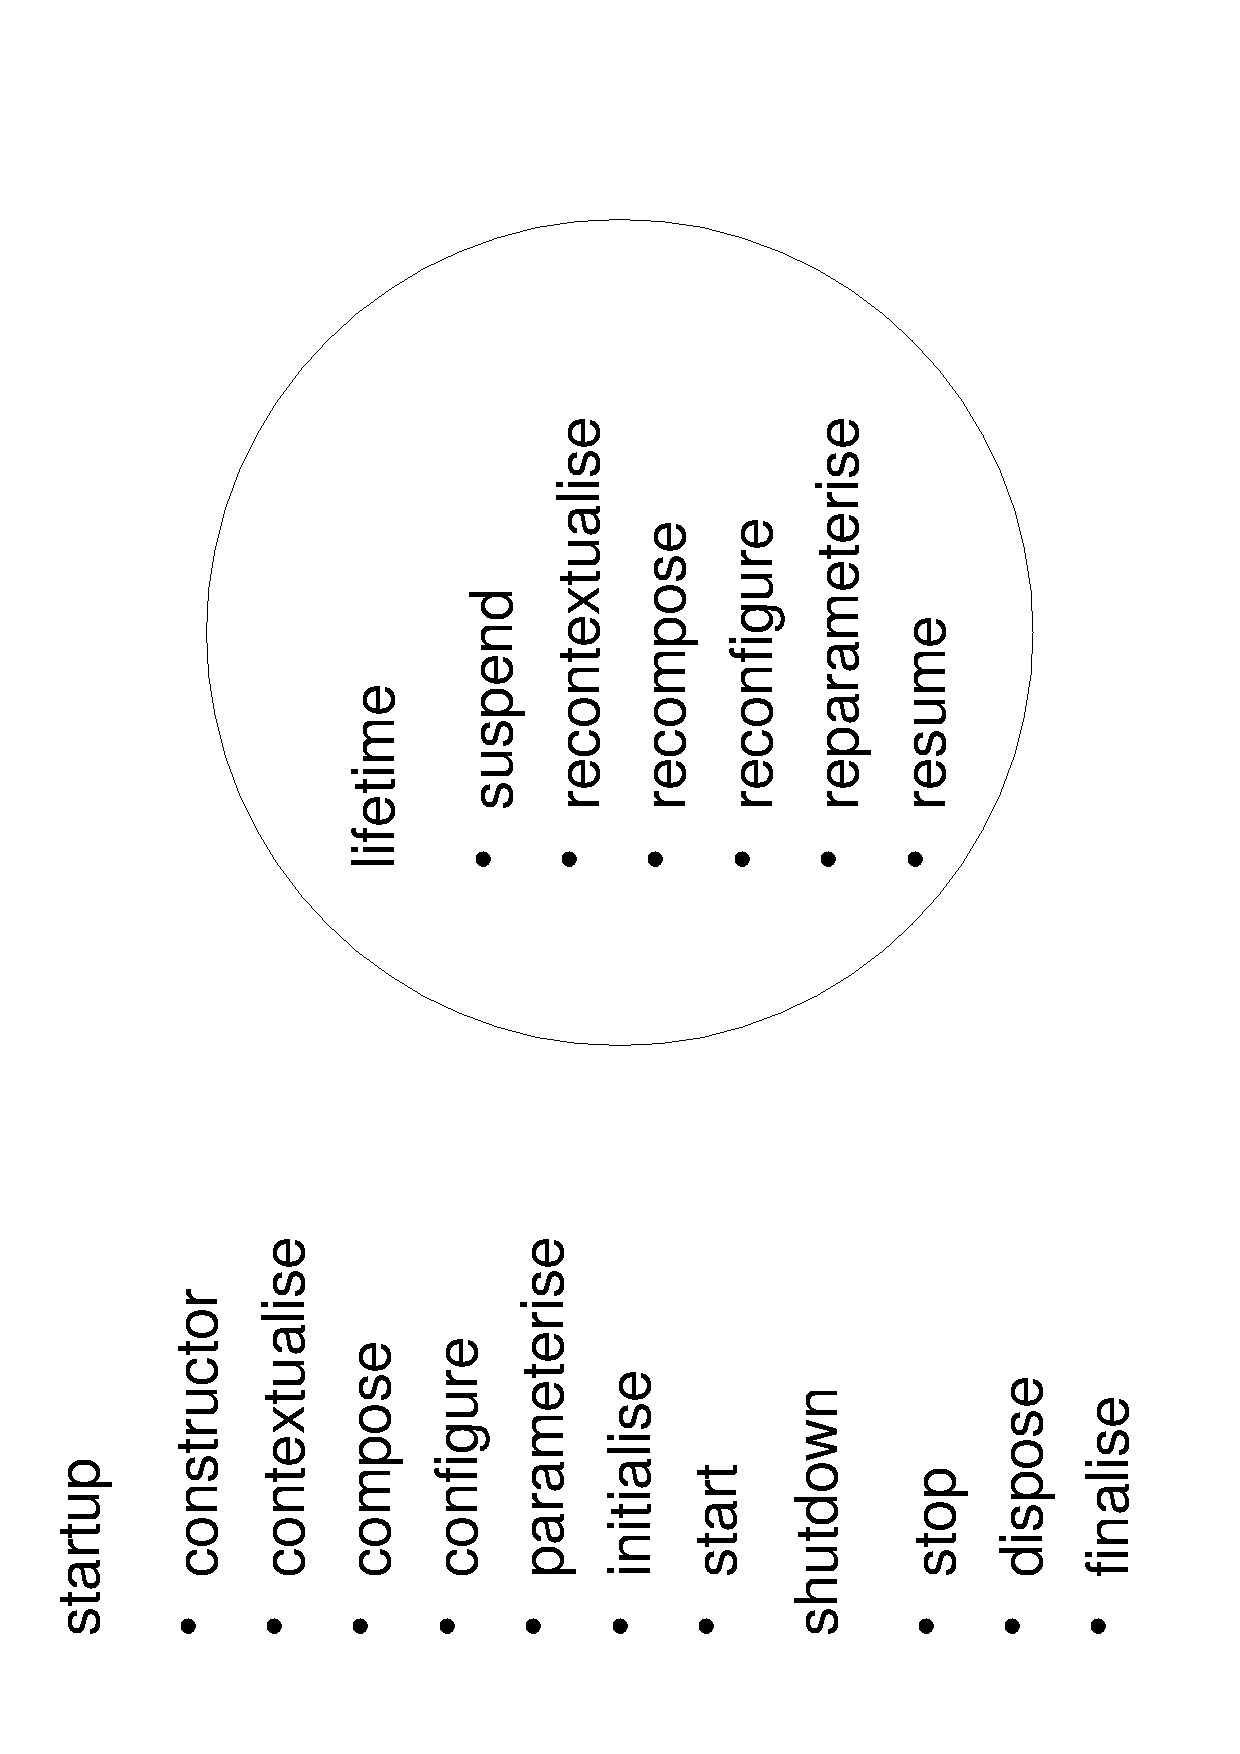
\includegraphics[scale=0.3,angle=-90]{graphic/lifecycle.pdf}
        \caption{Component Lifecycle Methods}
        \label{lifecycle_figure}
    \end{center}
\end{figure}

The lifecycle of a component specifies the methods that can be called on it,
and the order in which this may happen. The corresponding methods are called
\emph{Lifecycle Methods}. Some of them can be called only once in a specific
phase of a component's lifecycle, others may be called multiple times. The
methods in figure \ref{lifecycle_figure} are examples taken from the
\emph{Avalon} \cite{avalon} project. They represent three phases in a
component's lifecycle: \emph{Startup}, \emph{Lifetime} and \emph{Shutdown}.

Lifetime phase methods can be called repeatedly, at various times after startup
and before shutdown. The \emph{constructor} is called as a consequence of
instantiation. Its counterpart \emph{destructor} is not considered in the
project; since \emph{Avalon} is a Java-based framework, it was omitted because a
\emph{Garbage Collector} destroys instances at some indeterminate moment.

\textit{The order in which the various lifecycle methods are called is very
specific. While none are required (it is possible to have a component
implementing none of the lifecycle methods, although the use of that would be
limited), some can only be used when others are as well. It is up to each
container to indicate which lifecycle methods it will honour}, as \cite{avalon}
writes. This should be clearly documented together with the description of the
container.

A component lifecycle allows to forward parameters throughout a whole framework,
which makes static objects such as the singleton managers criticised in section
\ref{global_access_heading} superfluous. The \emph{configure} method, for
example, may forward a \emph{Configuration} object containing parameters that
otherwise would have to be made global.
